\documentclass[11pt,a4paper]{article}

\usepackage[utf8]{inputenc}
\usepackage[T1]{fontenc}
\usepackage{amsmath,amssymb,amsthm,mathtools}
\usepackage[margin=2.5cm]{geometry}
\usepackage{graphicx}
\usepackage{booktabs}
\usepackage{tabularx}
\usepackage{subcaption}
\usepackage{hyperref}
\usepackage{xcolor}
\usepackage{enumitem}

\hypersetup{colorlinks=true, linkcolor=blue!60!black, citecolor=blue!60!black, urlcolor=blue!60!black}

\newtheorem{remark}{Remark}
\newcommand{\R}{\mathbb{R}}
\newcommand{\loss}{\mathcal{L}}
\DeclareMathOperator*{\argmin}{arg\,min}
\DeclareMathOperator{\lammin}{\lambda_{\min}}

\title{One-Pass Deep Solvers for Stationary Hamilton--Jacobi--Bellman
Equations via Convexity Constraints and Homotopy Continuation\\[1ex]
\large Working paper --- experimental report}
\author{Alexis Laignelet}
\date{June 2026}

\begin{document}
\maketitle

\begin{abstract}
Physics-informed training of neural networks on the residual of a stationary
Hamilton--Jacobi--Bellman (HJB) equation reliably converges to
\emph{spurious solutions}: functions that satisfy the partial differential
equation to high accuracy but are not the value function of the underlying
optimal control problem. Prior work resolved this with a two-pass scheme,
first fitting the network to data generated from a State-Dependent Riccati
Equation (SDRE) approximation and then refining on the PDE residual. This
paper investigates whether the data pass can be removed entirely. We show
experimentally that (i)~hard architectural convexity (input-convex neural
networks, ICNNs) defines the correct solution class but is not trainable
through the residual loss on our benchmarks; (ii)~a soft hinge penalty on the
smallest Hessian eigenvalue of the \emph{output}, combined with a
strong-convexity margin and a data-free equilibrium anchor, recovers the
exact value function of a 2D linear-quadratic regulator (LQR) in a single
pass (evaluation MSE $2\times10^{-8}$); and (iii)~on a nonlinear benchmark
the same stack stalls in an optimization plateau, which is eliminated by
\emph{homotopy continuation} in the nonlinearity parameter, recovering the
true value function to MSE $6\times10^{-6}$ --- five orders of magnitude
better than any non-continuation variant and three orders better than the
SDRE warm start used as supervised data in the two-pass approach. The
resulting recipe --- resampled residual + convexity margin penalty +
equilibrium anchor + homotopy continuation --- uses no precomputed solution
data anywhere, and scales beyond closed-form eigenvalues: with a
directional-curvature penalty it solves a ten-dimensional nonlinear problem
with provably convex value function to $\approx 1\%$ relative error,
strictly convex at every audited point. We also delimit the method's scope:
a finite-difference study shows the Cucker--Smale flocking value function is
\emph{not} convex in the domain interior, so the convexity prior is
misspecified there. Finally we show the soft penalty is not the only
route: two architectures are convex \emph{by construction} over unconstrained
parameters and need no penalty --- a repaired ICNN (input skip connections
plus smooth positivity), where a controlled ablation shows the skip
connection alone moves LQR accuracy from $1.8\times10^{-2}$ to
$2.2\times10^{-7}$, and a log-sum-exp-of-quadratics network, exact on LQR
($3.6\times10^{-9}$). The ICNN's original failure traces to weight-space
constraint geometry, not to convexity itself. We document the full
experimental trail, including negative results, diagnostics, and the failure
modes of each ablated ingredient.
\end{abstract}

%=============================================================================
\section{Introduction}
%=============================================================================

The value function $V$ of an infinite-horizon optimal control problem
satisfies a stationary HJB equation. Solving this PDE with a neural network
trained on the squared residual --- the physics-informed neural network
(PINN) paradigm \cite{raissi2019physics} --- is attractive because it avoids
grid-based discretization. It suffers, however, from a structural problem:
on a bounded domain and without boundary conditions, the stationary HJB
equation does not have a unique solution \cite{bardi1997optimal}. Gradient
descent on the residual
loss happily converges to solution branches that have nothing to do with the
optimal control problem.

In earlier work \cite{borovykh2022data} we addressed this with a
\emph{two-pass} scheme: pass~1 fits the network to values and gradients of
an approximate solution obtained from the State-Dependent Riccati Equation
(SDRE) \cite{banks2007nonlinear}, placing the network in the basin of the
true solution; pass~2 minimizes the PDE residual to refine beyond the
accuracy of the SDRE data. The scheme works, but it requires generating
problem-specific data, and the SDRE machinery does not scale gracefully.

This paper asks: \textbf{can the data pass be replaced by structural
knowledge alone?} The structural facts available for a broad class of
problems are:
\begin{enumerate}[itemsep=1pt]
  \item the value function is \emph{convex} (e.g.\ LQR; and verified
        numerically for our nonlinear benchmark, Section~\ref{sec:nl-convex});
  \item the origin is the equilibrium: $V(0)=0$, $\nabla V(0)=0$;
  \item the problem family often interpolates continuously to a solvable
        base case (e.g.\ a nonlinearity parameter $\varepsilon$ with
        $\varepsilon=0$ giving LQR).
\end{enumerate}
None of these requires precomputing a solution.

\paragraph{Contributions.}
\begin{enumerate}[itemsep=1pt]
  \item A systematic negative result: skip-free ICNNs --- convex by
        construction --- cannot be trained through the HJB residual on our
        benchmarks. We trace the failure to two distinct mechanisms (dying
        units under weight clipping; a universal degenerate attractor) and
        show it persists across activations, initializations and training
        budgets (Section~\ref{sec:icnn}).
  \item A soft \emph{output-convexity} formulation: a differentiable hinge
        penalty on $\lammin(\nabla^2 V_\theta(x))$ with a strong-convexity
        margin, which acts as a solution-selection mechanism and solves the
        LQR benchmark exactly in one pass (Section~\ref{sec:soft}).
  \item The identification of a residual optimization plateau on the
        nonlinear benchmark --- after eliminating, via targeted diagnostics,
        every competing explanation (feasibility, capacity, collocation
        overfitting, evaluation artefacts) --- and its resolution by homotopy
        continuation in the nonlinearity (Section~\ref{sec:continuation}).
  \item A scaling of the recipe to ten dimensions: a directional-curvature
        penalty replaces the closed-form 2D eigenvalue, solving a 10D
        nonlinear problem with provably convex value function to
        $\approx 1\%$ relative error, strictly convex at every audited
        point; and a scope result showing the Cucker--Smale flocking value
        function is non-convex in the domain interior, so the convexity
        prior does not apply there (Section~\ref{sec:highdim}).
  \item Two certified, penalty-free alternatives, with a diagnosis of why the
        skip-free ICNN fails (weight-space constraint geometry, not the
        convexity property): (a) a \emph{repaired ICNN} --- input skip
        connections plus smooth positivity --- where a controlled ablation
        shows the skip connection alone moves LQR from $1.8\times10^{-2}$ to
        $2.2\times10^{-7}$; and (b) a log-sum-exp-of-quadratics architecture,
        $m$-strongly convex by construction over unconstrained parameters and
        exact on LQR ($3.6\times10^{-9}$). Both solve all benchmarks
        convex-by-construction with no penalty term (Section~\ref{sec:lseq}).
  \item A complete ablation trail showing each ingredient of the final
        recipe is necessary, together with a candid pros-and-cons analysis
        of all approaches tried (Section~\ref{sec:discussion}).
\end{enumerate}

%=============================================================================
\section{Problem setting}\label{sec:setting}
%=============================================================================

We consider control-affine dynamics and quadratic control cost,
\begin{equation}
  \dot y = f(y) + g(y)\,u, \qquad
  J = \int_0^\infty \big( \ell(y(t)) + \beta \|u(t)\|^2 \big)\,dt,
\end{equation}
whose value function satisfies the stationary HJB equation
\begin{equation}\label{eq:hjb}
  \mathcal{R}[V](x) \;:=\;
  \langle \nabla V(x), f(x)\rangle
  \;-\; \tfrac{1}{4\beta}\, \nabla V(x)^\top g(x) g(x)^\top \nabla V(x)
  \;+\; \ell(x) \;=\; 0 ,
\end{equation}
with optimal feedback $u^*(x) = -\tfrac{1}{2\beta} g(x)^\top \nabla V(x)$.
Note that \eqref{eq:hjb} involves only $\nabla V$; the value function is
determined up to an additive constant, which we fix by evaluation-time shift
correction or by the equilibrium anchor below.

\paragraph{Benchmarks.} Two problems on the domain $[-1,1]^2$:
\begin{itemize}[itemsep=1pt]
  \item \textbf{LQR2D}: $f(x)=Ax$, $g=B$, $\ell(x)=\tfrac12 x^\top Q x$,
        with known analytic solution $V^*(x) = \tfrac12 x^\top P x$,
        $P = \tfrac15(1+\sqrt6)\,I$ (Hessian floor $\approx 0.69$).
  \item \textbf{NonLinear2D}: $\dot y_0 = y_1$, $\dot y_1 = \varepsilon
        y_0^3 + u$ with $\varepsilon = 1$, $\beta = \tfrac12$,
        $\ell(x) = \tfrac12\|x\|^2$. Ground truth on a $100\times100$ grid
        from the prior work's converged solver; values in $[0, 5.7]$.
\end{itemize}

\paragraph{Spurious solutions.} On a bounded domain without boundary
conditions, \eqref{eq:hjb} admits multiple solutions; for LQR both Riccati
branches solve the PDE, and only the stabilizing (convex) branch is the
value function. This is the central difficulty: \emph{a small residual does
not certify the right solution}. Empirically, an unconstrained network
trained on the residual of LQR2D reaches residual $4.7\times10^{-8}$ while
its evaluation error against the true value function remains at
$4.6\times10^{-2}$ (Table~\ref{tab:lqr}); the same phenomenon appears on
NonLinear2D, where the expected residual reaches $2.3\times10^{-5}$ at
evaluation error $1.2$ (Table~\ref{tab:nl}), and the learned surface is
visibly a different object from the value function
(Figure~\ref{fig:nl-surfaces}).

\paragraph{Network, loss, and protocol.} Unless stated otherwise the
network is a multilayer perceptron with three hidden layers of width~32.
The base loss is the mean squared residual at $n=500$ interior collocation
points. Training uses Adam with a staged learning-rate schedule
($10^{-2}\!\to\!10^{-5}$, 10k--28k epochs). Evaluation reports the MSE
against the ground truth on a $100\times100$ grid (shift-corrected for
residual-only runs), and convexity of the \emph{learned network} is verified
post hoc by the exact autograd Hessian on a $20\times20$ grid: we report the
global minimum eigenvalue and the fraction of grid points violating positive
semi-definiteness.

%=============================================================================
\section{Route 1: hard architectural convexity (ICNN)}\label{sec:icnn}
%=============================================================================

Input-convex neural networks \cite{amos2017input} guarantee convexity by
construction: all weights after the first layer are constrained non-negative
and activations must be convex and non-decreasing. We tested the skip-free
variant with the principled initialization of \cite{hoedt2023principled},
several positivity mechanisms (lazy clipping, exponential reparameterization,
and their no-positivity ablations), and a sweep of convexity-safe activations
(ReLU, Softplus, ELU, CELU, LeakyReLU).

\paragraph{Failure mechanism 1: dying units under clipping.} With ReLU, the
combination of non-negative weights and the negative biases installed by the
convex initializer kills hidden units: in the trained network 25/32 units of
the second layer and \emph{31/32 units of the third layer} are dead
(pre-activation negative on the whole domain), and the loss gradient is
exactly zero for every parameter except the output layer. Training stalls
within a few hundred steps.

\paragraph{Failure mechanism 2: a universal degenerate attractor.} Several
distinct configurations (LeakyReLU; Softplus with standard initialization;
a wider Softplus network) collapse to \emph{bit-identical} final losses
($1.57\times10^{-1}$) --- the same degenerate, nearly-affine function.

\paragraph{Best case still underfits.} Smooth convex activations with the
convex initializer do train and are \emph{strictly} convex (positive minimum
Hessian eigenvalue), but the residual plateaus near $6\times10^{-3}$ ---
three orders above what unconstrained networks reach --- and tripling the
training budget changes nothing (Table~\ref{tab:lqr}, rows 5--6;
Figure~\ref{fig:icnn-underfit}).

\begin{remark}
Two caveats temper this negative result. First, a ReLU network is piecewise
linear, so its Hessian is zero almost everywhere: the convexity check passes
\emph{vacuously} and the architecture contributes no useful curvature
signal. Second, our ICNN lacks the input passthrough (skip) connections of
the original architecture, which are also what make ICNNs universal over
convex functions; the failure reported here is for the skip-free variant.
\end{remark}

\begin{figure}[t]
  \centering
  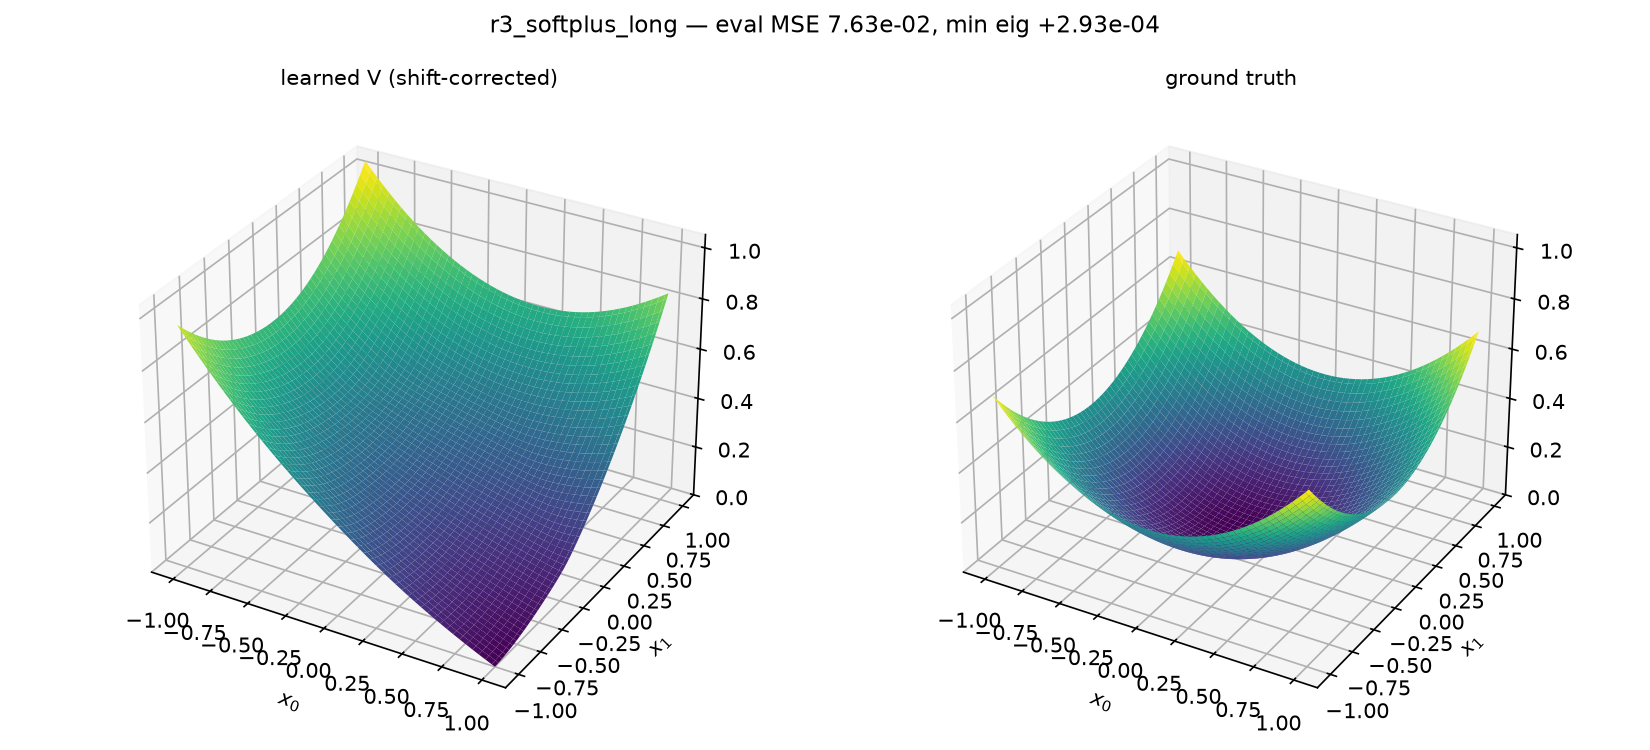
\includegraphics[width=0.95\textwidth]{figures/icnn_underfit.png}
  \caption{Best hard-ICNN configuration on LQR2D (Softplus, clipping, convex
  initialization, $3\times$ budget): strictly convex but underfitted
  (eval.\ MSE $7.6\times10^{-2}$) --- the architectural route defines the
  right class but cannot navigate to the right element of it.}
  \label{fig:icnn-underfit}
\end{figure}

%=============================================================================
\section{Route 2: soft output convexity}\label{sec:soft}
%=============================================================================

Rather than constraining weights, we penalize non-convexity of the
\emph{output}. In 2D the smallest Hessian eigenvalue has a closed form: with
$H = \nabla^2 V_\theta(x)$, $a = H_{11}$, $b = H_{12}$, $c = H_{22}$,
\begin{equation}
  \lammin(x) \;=\; \tfrac12 (a + c) - \sqrt{\tfrac14 (a-c)^2 + b^2},
\end{equation}
which is differentiable and assembled from one extra back-propagation
through $\nabla V_\theta$ (already computed for the residual). The training
loss becomes
\begin{equation}\label{eq:loss}
  \loss(\theta) \;=\;
  \underbrace{\frac1n \sum_{i} \mathcal{R}[V_\theta](x_i)^2}_{\text{residual}}
  \;+\; w \,\underbrace{\frac1n \sum_{i} \max\!\big(0,\; m - \lammin(x_i)\big)}_{\text{convexity hinge, margin } m}
  \;+\; a \,\underbrace{\big( V_\theta(0)^2 + \|\nabla V_\theta(0)\|^2 \big)}_{\text{equilibrium anchor}} .
\end{equation}
The three ingredients encode, respectively: the PDE; convexity with a
\emph{strong-convexity margin} $m$ (require $\lammin \ge m$, chosen below
the true solution's curvature floor); and the equilibrium conditions
$V(0)=0$, $\nabla V(0)=0$, which are problem knowledge, not data. Interior
points are \emph{resampled at every step}, so the loss targets the expected
residual rather than a fixed collocation set. We also implemented an
augmented-Lagrangian treatment of the constraint $\lammin(x)\ge m$
(per-point multipliers on a fixed $20\times20$ grid) as an alternative to
the fixed-weight hinge.

\subsection{Results on LQR2D}

Table~\ref{tab:lqr} summarizes the progression. The decisive ingredient is
the margin: the plain hinge ($m=0$) improves the evaluation error tenfold
over the unconstrained baseline, but the margin $m = 0.1$ --- comfortably
below the true curvature floor $0.69$, excluding the concave spurious branch
entirely --- recovers the analytic Riccati solution to machine-practical
accuracy: evaluation MSE $1.7\times10^{-7}$, strictly convex on the whole
domain. Robust across seeds ($2.7\times10^{-6}$, $7.7\times10^{-8}$), and
the equilibrium anchor improves it further to $2.1\times10^{-8}$.
Figure~\ref{fig:lqr-surfaces} shows the learned surfaces.

\begin{table}[t]
\centering\small
\caption{LQR2D, one-pass residual-only training (seed 0 unless noted).
``Viol.'' is the fraction of test-grid points where the learned Hessian has
a negative eigenvalue.}
\label{tab:lqr}
\setlength{\tabcolsep}{2.5pt}
\begin{tabular}{lcccc}
\toprule
Configuration & Residual & Eval.\ MSE & $\min\lammin$ & Viol. \\
\midrule
Unconstrained MLP (Sigmoid)            & $1.5\times10^{-5}$ & $4.4\times10^{-2}$ & $-0.46$ & 100\% \\
Unconstrained MLP (GELU)               & $4.7\times10^{-8}$ & $4.6\times10^{-2}$ & $-0.29$ & 100\% \\
ICNN, ReLU + clipping                  & $1.6\times10^{-1}$ & $7.7\times10^{-2}$ & $0.0$   & 0\%\,(vacuous) \\
ICNN, Softplus + exp.\ weights         & $5.7\times10^{2}$  & $9.7\times10^{-1}$ & $+1.05$ & 0\% \\
ICNN, CELU + clipping + convex init    & $6.6\times10^{-3}$ & $9.1\times10^{-2}$ & $+1.9\times10^{-4}$ & 0\% \\
ICNN, Softplus, $3\times$ budget       & $6.0\times10^{-3}$ & $7.6\times10^{-2}$ & $+2.9\times10^{-4}$ & 0\% \\
\midrule
Hinge penalty $w{=}1$, $m{=}0$         & $1.6\times10^{-4}$ & $4.9\times10^{-3}$ & $-1.67$ & 2\% \\
Hinge penalty $w{=}1$, $m{=}0.1$       & $1.9\times10^{-7}$ & $\mathbf{1.7\times10^{-7}}$ & $+0.60$ & 0\% \\
\quad same, seed 1 / seed 2            & --- & $2.7\times10^{-6}$ / $7.7\times10^{-8}$ & $>0$ & 0\% \\
\quad + equilibrium anchor             & $2.8\times10^{-7}$ & $\mathbf{2.1\times10^{-8}}$ & $+0.62$ & 0\% \\
\bottomrule
\end{tabular}
\end{table}

\begin{figure}[t]
  \centering
  \begin{subfigure}[b]{0.95\textwidth}
    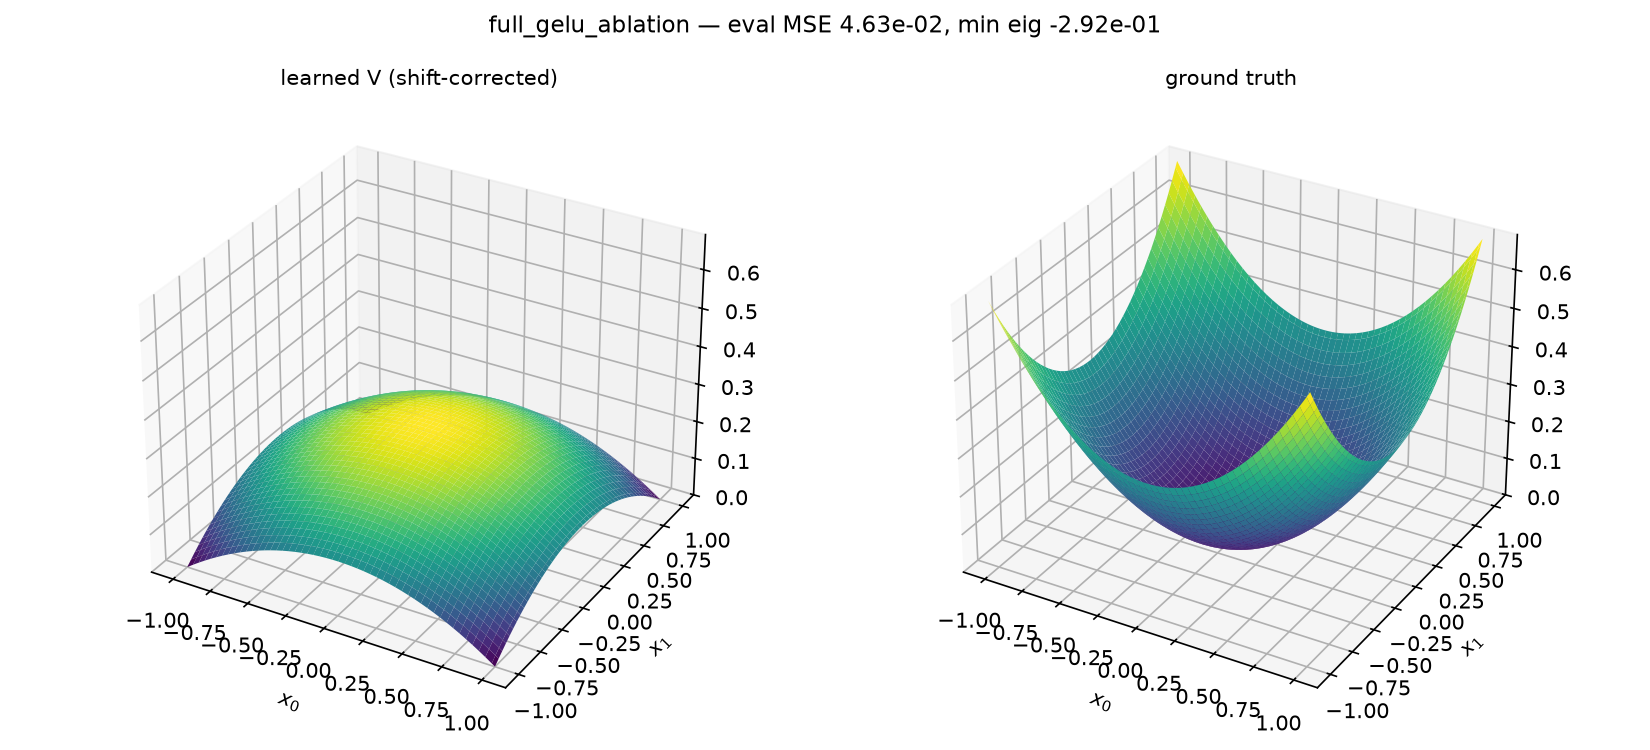
\includegraphics[width=\textwidth]{figures/lqr_spurious.png}
    \caption{Unconstrained GELU network: residual $4.7\times10^{-8}$, yet the
    learned surface (left) is a spurious solution, far from the truth (right).}
  \end{subfigure}\\[1ex]
  \begin{subfigure}[b]{0.95\textwidth}
    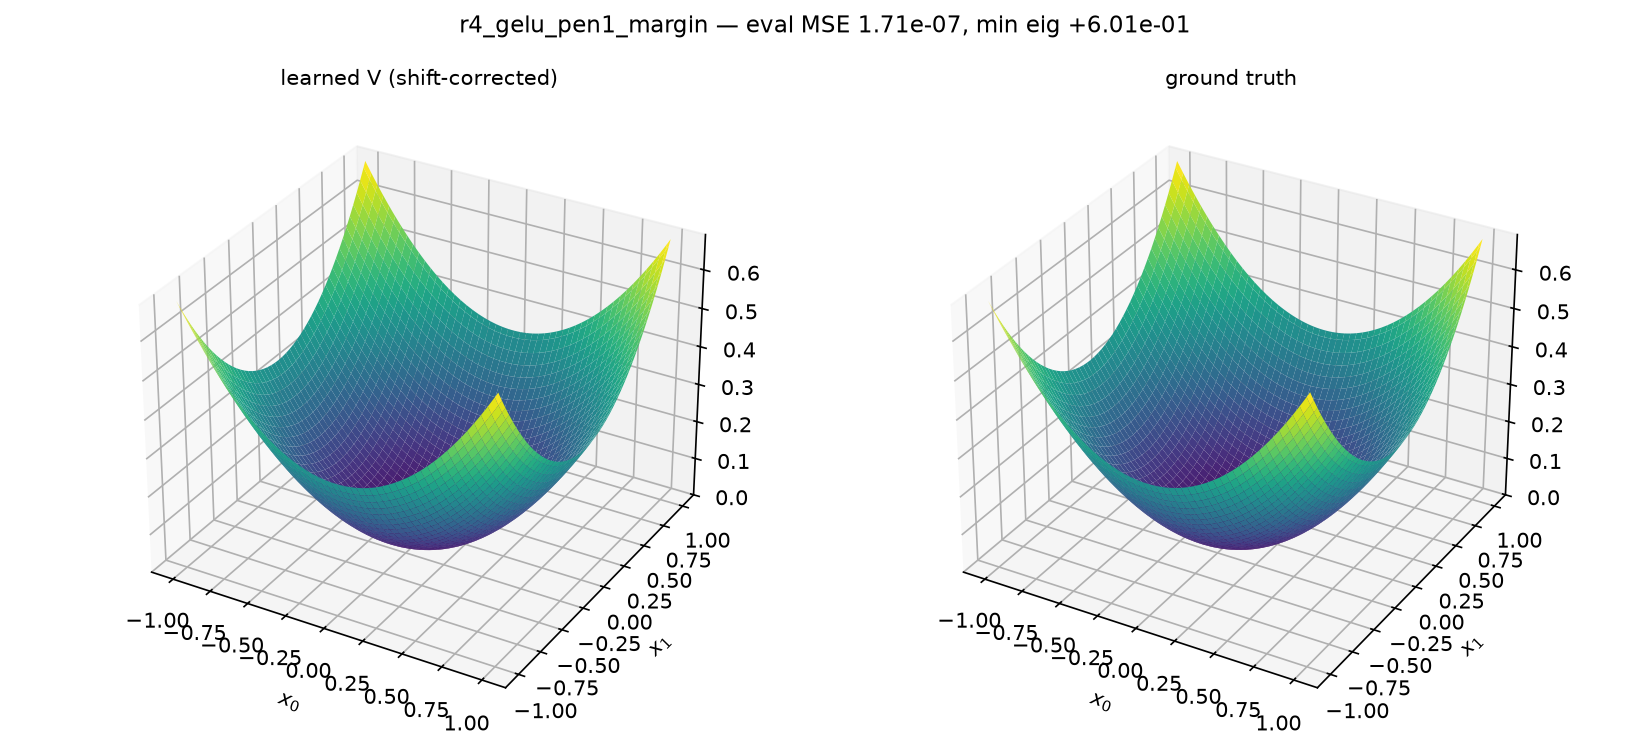
\includegraphics[width=\textwidth]{figures/lqr_solved.png}
    \caption{Same network with the convexity hinge and margin $m=0.1$: the
    exact Riccati value function is recovered (eval.\ MSE $1.7\times10^{-7}$).}
  \end{subfigure}
  \caption{LQR2D learned value functions (left panels) vs ground truth
  (right panels).}
  \label{fig:lqr-surfaces}
\end{figure}

%=============================================================================
\section{The nonlinear benchmark: diagnostics and continuation}
\label{sec:continuation}
%=============================================================================

Transferring the stack to NonLinear2D initially failed: every configuration
--- unconstrained, hinge, augmented Lagrangian, with or without anchor ---
landed at evaluation error $\approx 1.2$. Before changing the method we
eliminated the competing explanations one by one.

\subsection{Is the convex ansatz even well-specified?}\label{sec:nl-convex}
A finite-difference Hessian analysis of the ground-truth grid shows the true
value function \emph{is} convex --- minimum eigenvalue $\ge 0.02$
everywhere, median $0.73$. (Our first margin guess $m=0.05$ exceeded the
floor $0.02$ in places and was infeasible; all subsequent runs use
$m = 0.01$.)

\subsection{Is the evaluation sound?}
A supervised control fit exposed a long-standing \textbf{evaluation bug}:
the ground-truth grid was flattened without transposing, mismatching the
orientation of the evaluation points; every historical evaluation error on
this benchmark was computed against a transposed surface. We verified the
correct orientation against the analytic SDRE formula (mismatch MSE $0.108$
as stored vs $0.0076$ transposed), fixed the loader, and re-scored all
saved models. After the fix, the supervised fit scores $8.6\times10^{-3}$,
essentially the SDRE's own $7.6\times10^{-3}$ gap to the truth (the small
excess is network fit error), confirming the pipeline. The
residual-only runs remain at $\approx 1.2$: genuinely spurious.

\subsection{Is it feasible, representable, or overfitted?}
Three facts pin the failure down to optimization:
\begin{itemize}[itemsep=1pt]
  \item \textbf{Feasibility}: the ground truth satisfies the coded residual
        to MSE $3.4\times10^{-7}$ (finite differences), so ``convex +
        residual $\approx 0$ + anchored'' is achievable.
  \item \textbf{Capacity}: the same architecture fits the ground truth
        \emph{supervised} to MSE $3.7\times10^{-6}$; the truth-fitted
        network's own residual is $1.2\times10^{-3}$.
  \item \textbf{Collocation overfitting}: the unconstrained network's
        residual degrades $100\times$ off its fixed 500 training points
        ($5\times10^{-6} \to 5\times10^{-4}$). Per-step resampling removes
        the overfit but does \emph{not} remove the spurious branch: with
        resampling the expected residual still reaches $2.3\times10^{-5}$
        at evaluation error $1.20$ --- the spurious branch is a genuine
        alternative (near-)solution of the PDE, not an artefact.
\end{itemize}
Under the convexity constraint, every optimizer variant (fixed hinge,
augmented Lagrangian, data-free warm shaping to a quadratic bowl, all
budgets) converges to the \emph{same} convex non-solution: residual stuck at
$\approx 3\times10^{-2}$, minimum eigenvalue pinned at the margin
(Figure~\ref{fig:nl-surfaces}, middle row). The truth (curvature floor
$0.02$, residual $3.4\times10^{-7}$) is feasible and strictly inside the
constraint --- the obstacle is purely the optimization landscape.

\subsection{Homotopy continuation in the nonlinearity}
The problem family interpolates to a solvable base case: at $\varepsilon=0$
the dynamics are linear and the problem is an LQR, which the one-pass stack
solves exactly. We therefore anneal $\varepsilon$ from $0$ to $1$ over the
first 12k of 28k training steps, tracking the continuous solution path
$V(\varepsilon)$ --- a numerical-continuation strategy
\cite{allgower1990numerical} --- instead of attacking the $\varepsilon=1$
landscape cold.

The effect is decisive (Table~\ref{tab:nl}): evaluation error drops from
$1.2$ to $5.9\times10^{-6}$ (hinge variant) and $8.9\times10^{-6}$
(augmented-Lagrangian variant) --- five orders of magnitude --- and the
learned curvature floor ($+0.0202$) lands exactly on the measured floor of
the true solution ($0.02$). Figure~\ref{fig:nl-surfaces} (bottom) shows the
learned surface is visually indistinguishable from the truth.

\begin{table}[t]
\centering\small
\caption{NonLinear2D, corrected evaluation. All rows except the supervised
control are one-pass residual-only (no solution data). ``Stack'' = resampled
residual + hinge $w{=}10$, $m{=}0.01$ + anchor $a{=}10$.}
\label{tab:nl}
\begin{tabular}{lcccc}
\toprule
Configuration & Residual & Eval.\ MSE & $\min\lammin$ & Viol. \\
\midrule
Supervised control (fits SDRE data)        & ---                & $8.6\times10^{-3}$ & $-0.53$ & 4\% \\
\midrule
Unconstrained, resampled                   & $2.3\times10^{-5}$ & $1.20$ & $-27.9$ & 84\% \\
Stack, no continuation                     & $3.4\times10^{-2}$ & $1.25$ & $+9.9\times10^{-3}$ & 0\% \\
Stack, augmented Lagrangian                & $3.3\times10^{-2}$ & $1.25$ & $+8.7\times10^{-3}$ & 0\% \\
Stack + warm shaping                       & $2.6\times10^{-2}$ & $1.19$ & $+7.9\times10^{-3}$ & 0\% \\
\midrule
\textbf{Stack + $\varepsilon$-continuation}         & $1.1\times10^{-5}$ & $\mathbf{5.9\times10^{-6}}$ & $+0.0202$ & 0\% \\
AL variant + $\varepsilon$-continuation             & $5.6\times10^{-6}$ & $8.9\times10^{-6}$ & $+0.0098$ & 0\% \\
\bottomrule
\end{tabular}
\end{table}

\begin{figure}[t]
  \centering
  \begin{subfigure}[b]{0.95\textwidth}
    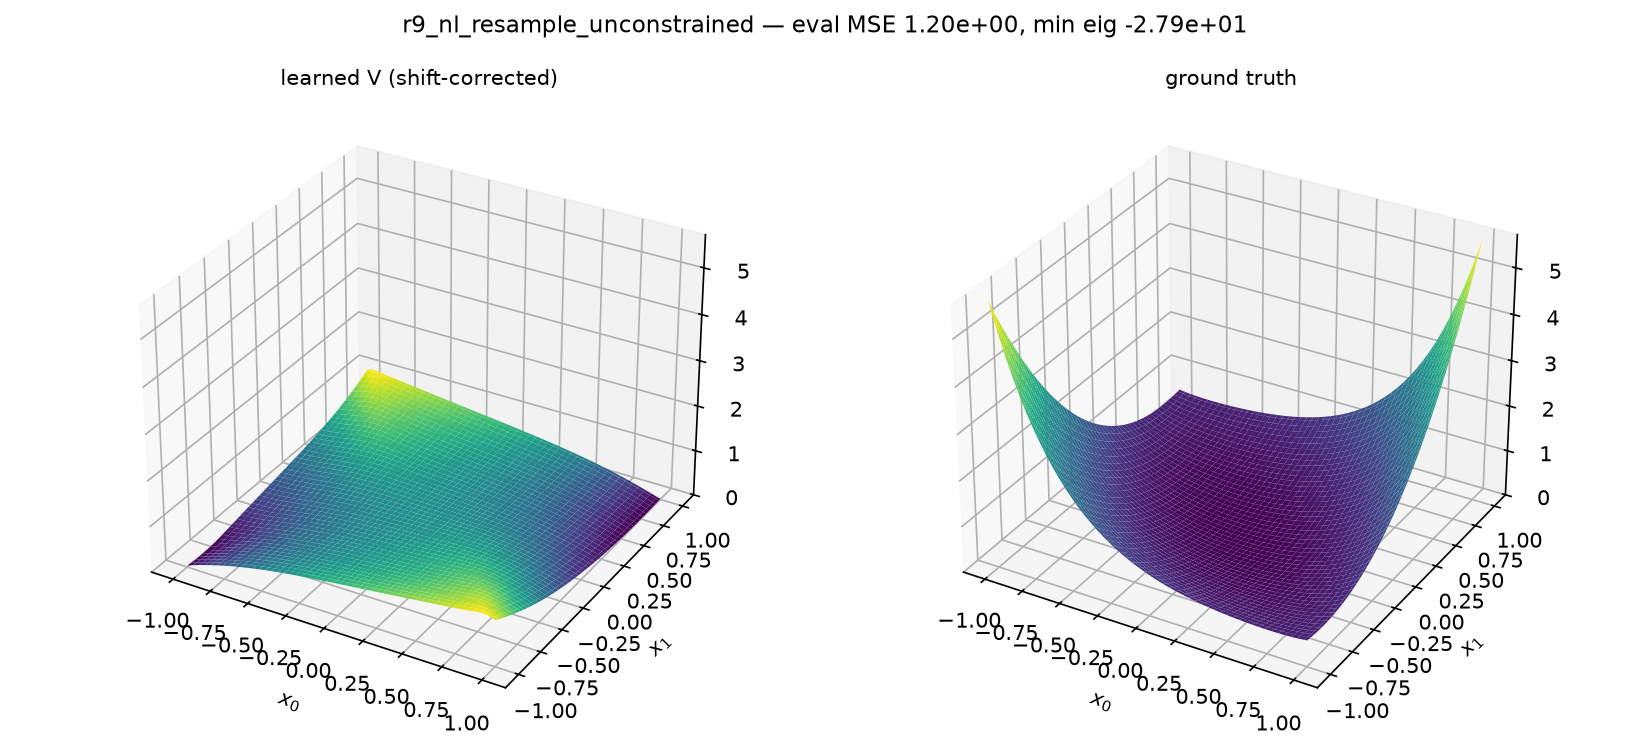
\includegraphics[width=\textwidth]{figures/nl_spurious.png}
    \caption{Unconstrained, resampled: expected residual $2.3\times10^{-5}$,
    but the learned surface is a spurious branch (eval.\ MSE $1.20$).}
  \end{subfigure}\\[1ex]
  \begin{subfigure}[b]{0.95\textwidth}
    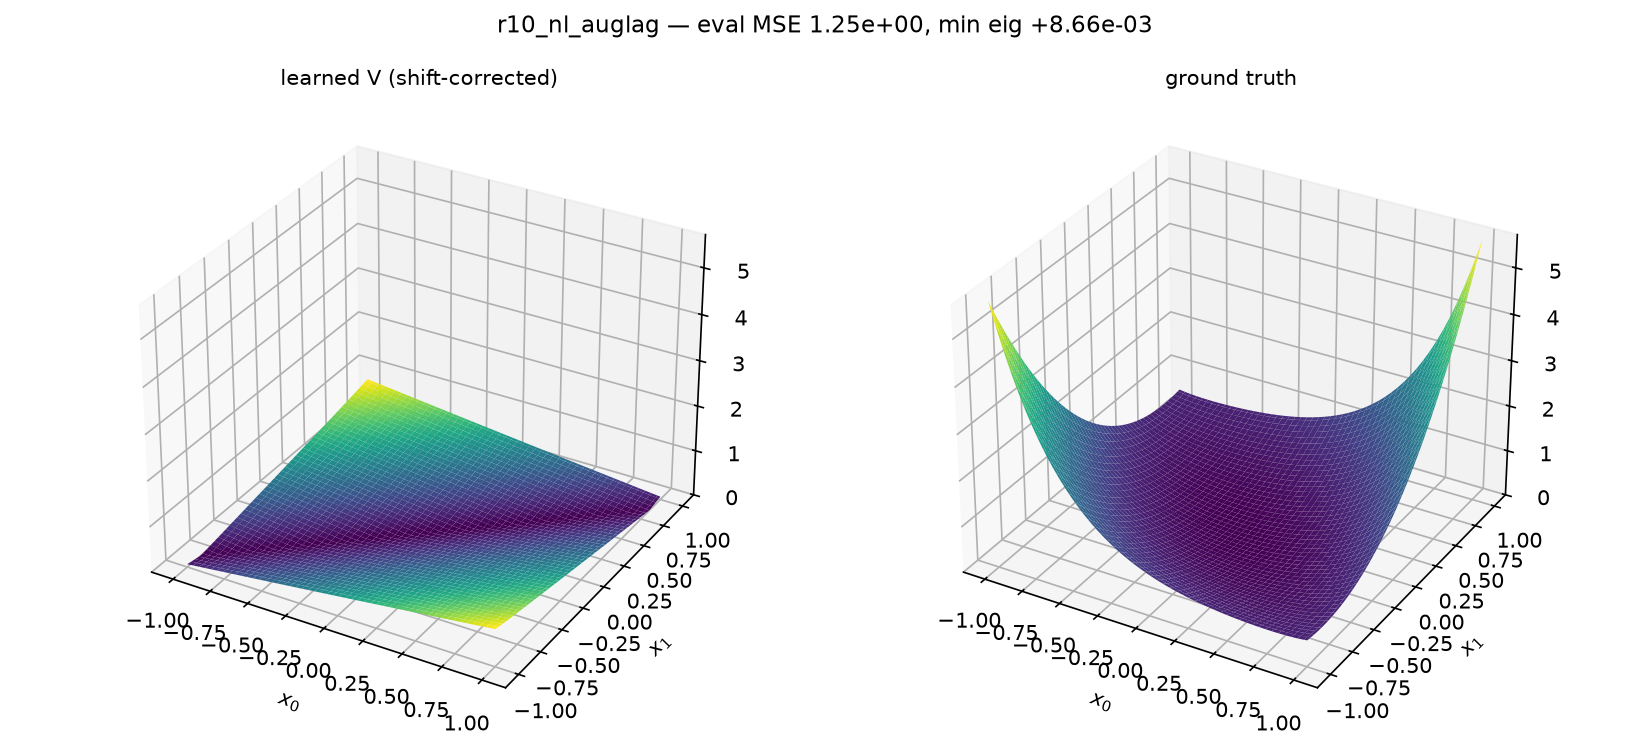
\includegraphics[width=\textwidth]{figures/nl_wall.png}
    \caption{Convexity-constrained without continuation: convex but stuck
    (residual $3\times10^{-2}$, eval.\ MSE $1.25$).}
  \end{subfigure}\\[1ex]
  \begin{subfigure}[b]{0.95\textwidth}
    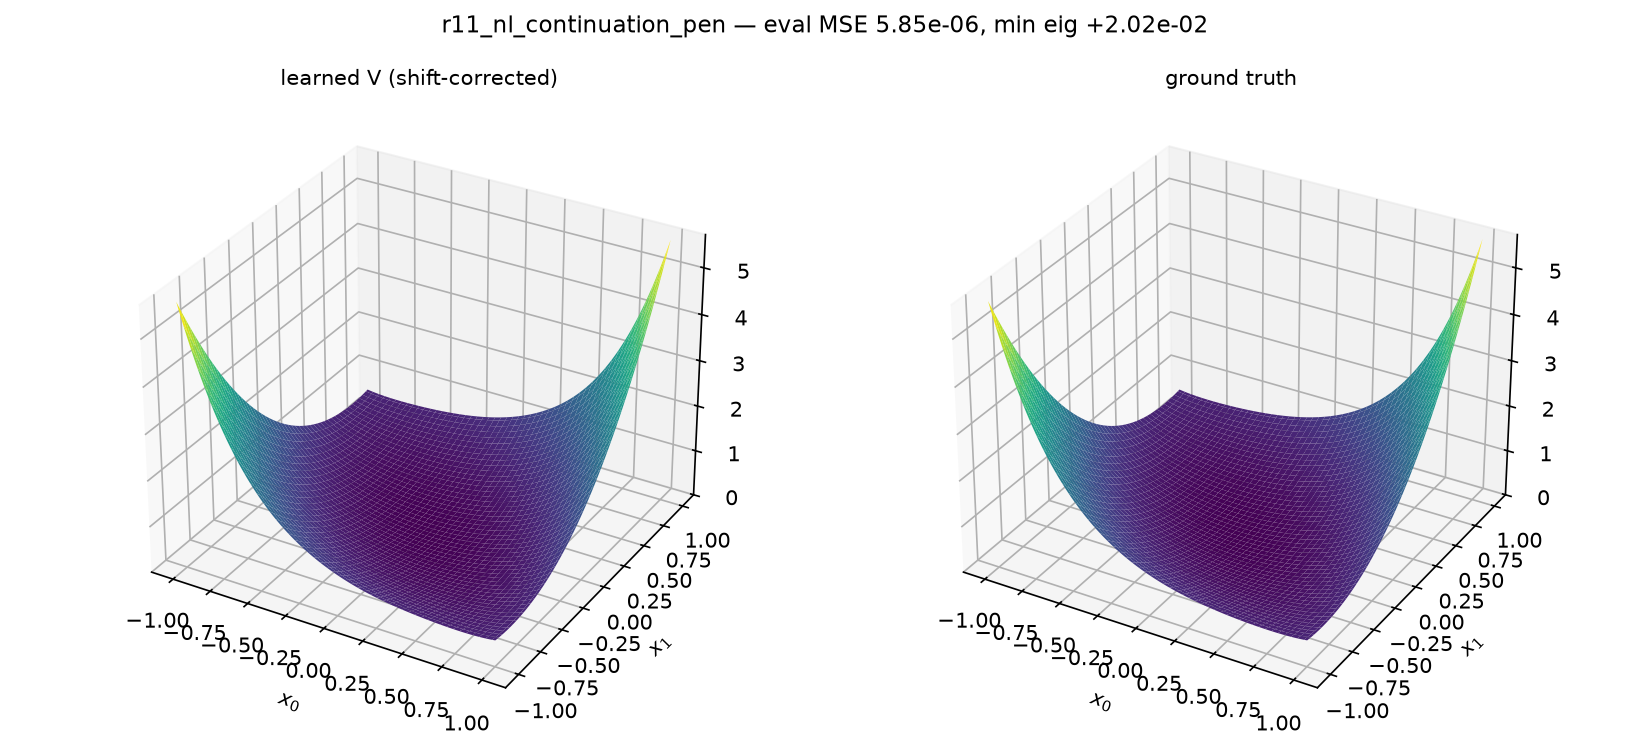
\includegraphics[width=\textwidth]{figures/nl_solved.png}
    \caption{Full stack with $\varepsilon$-continuation: the true value
    function is recovered (eval.\ MSE $5.9\times10^{-6}$).}
  \end{subfigure}
  \caption{NonLinear2D learned value functions (left panels) vs ground truth
  (right panels).}
  \label{fig:nl-surfaces}
\end{figure}

%=============================================================================
\section{Beyond two dimensions: scope and scaling}\label{sec:highdim}
%=============================================================================

\subsection{When the convexity prior does not apply: Cucker--Smale}
\label{sec:cs}

The Cucker--Smale flocking model (state = particle positions and velocities;
interaction kernel $a(y_i, y_j) = (1 + (y_i - y_j)^2)^{-1}$; consensus cost)
is the high-dimensional benchmark of our earlier work, and the natural next
target. Before applying the method we asked whether its value function is
convex at all. A 2024 study had found non-convex points of an SDRE-rollout
approximation of $V$, but only near the domain boundary and with a fragile
one-sided stencil --- possibly artefacts.

We redid the analysis on the interior: 150 random points in $[-2,2]^4$
(two particles, 4D state, domain $[-3,3]^4$), central differences with
$h = 0.05$ on the SDRE-rollout value. The result is unambiguous:
\textbf{4.7\% of interior points are non-convex, with minimum Hessian
eigenvalue down to $-0.25$} against a median curvature of $+0.34$, and the
violations lie well inside the domain ($|$positions$| \le 1.3$,
$|$velocities$| \le 1.8$). The worst point pairs separated positions with
opposing velocities --- precisely where the non-convex interaction kernel is
active. (Caveat: the SDRE rollout approximates $V$; this is strong evidence,
not proof.)

Two consequences. First, the convexity prior is \emph{misspecified} for
Cucker--Smale on this domain: a method that enforces convexity cannot
converge to its value function, which retroactively explains why the 2024
ICNN experiments on this problem could not have succeeded regardless of
trainability. Second, the method's scope claim must be: problems whose value
function is convex on the domain of interest --- a property that, as here,
can be checked numerically in advance. Extensions to Cucker--Smale would
require a convexity-region restriction (e.g.\ near the consensus manifold)
or a convex-plus-correction decomposition; both are open.

\subsection{A ten-dimensional benchmark with provably convex value function}
\label{sec:nd}

To test the recipe in higher dimension on a \emph{well-specified} problem,
we construct one whose value function is provably convex with an exact
ground truth. Take coordinate-wise dynamics and cost
\begin{equation}
  \dot y_i = \varepsilon y_i^3 + u_i, \qquad
  \ell(y) = \tfrac12 \|y\|^2, \qquad \beta = \tfrac12, \qquad
  y \in [-1,1]^{10}.
\end{equation}
The HJB equation decouples into scalar problems with closed-form stabilizing
solution
\begin{equation}
  v'(s) \;=\; 2\beta\varepsilon s^3 + s \sqrt{4\beta^2 \varepsilon^2 s^4 + 2\beta},
  \qquad
  v''(s) \;=\; 6\beta\varepsilon s^2 + \sqrt{\cdot}
  + \frac{8\beta^2\varepsilon^2 s^4}{\sqrt{\cdot}} \;>\; 0,
\end{equation}
where $\sqrt{\cdot}$ abbreviates the root $\sqrt{4\beta^2\varepsilon^2 s^4 +
2\beta}$ appearing in $v'$. Thus $V^*(x) = \sum_i v(x_i)$ is strictly convex
with curvature floor
$\sqrt{2\beta} = 1$ on all of $\R^{10}$ (margin $m = 0.1$ provably
feasible), and the ground truth is available by one-dimensional quadrature.
The network is a generic 10D MLP ($64\times3$, GELU); nothing in the method
exploits the decoupling.

Two ingredients must scale. The closed-form $2\times2$ eigenvalue is
replaced by a \emph{directional-curvature hinge}: at each step, for each
collocation point, draw $k=4$ random unit directions $v$ and penalize
$\max(0,\, m - v^\top \nabla^2 V_\theta(x)\, v)$, where $v^\top H v$ costs
one extra backpropagation through $\nabla V_\theta$. Since
$v^\top H v \ge \lammin$, with resampled points and directions this enforces
the spectral constraint in expectation. The post-hoc audit computes full
autograd Hessians and exact eigenvalues at 300 random points. Continuation
anneals $\varepsilon$ from 0 (a decoupled 10D LQR) to 1 over the first 12k
of 28k steps, as in Section~\ref{sec:continuation}.

\begin{table}[t]
\centering\small
\caption{10D benchmark, one-pass residual-only (no solution data). Eval.\
MSE against the quadrature ground truth on 5000 random points; Hessian
statistics from exact eigendecompositions at 300 random points. Typical
value magnitude is $\approx 3$, so MSE $1.7\times10^{-3}$ corresponds to
$\approx 1\%$ relative error.}
\label{tab:nd}
\setlength{\tabcolsep}{2pt}
\begin{tabular}{lcccc}
\toprule
Configuration & Residual & Eval.\ MSE & $\min\lammin$ & Viol. \\
\midrule
Unconstrained (no penalty/anchor/continuation) & $7.0\times10^{-6}$ & $1.53$ & $-1.03$ & 100\% \\
\textbf{Full stack (dir.\ curvature, $m{=}0.1$, anchor, continuation)} & $4.0\times10^{-3}$ & $\mathbf{1.7\times10^{-3}}$ & $+0.61$ & 0\% \\
\bottomrule
\end{tabular}
\end{table}

\begin{figure}[t]
  \centering
  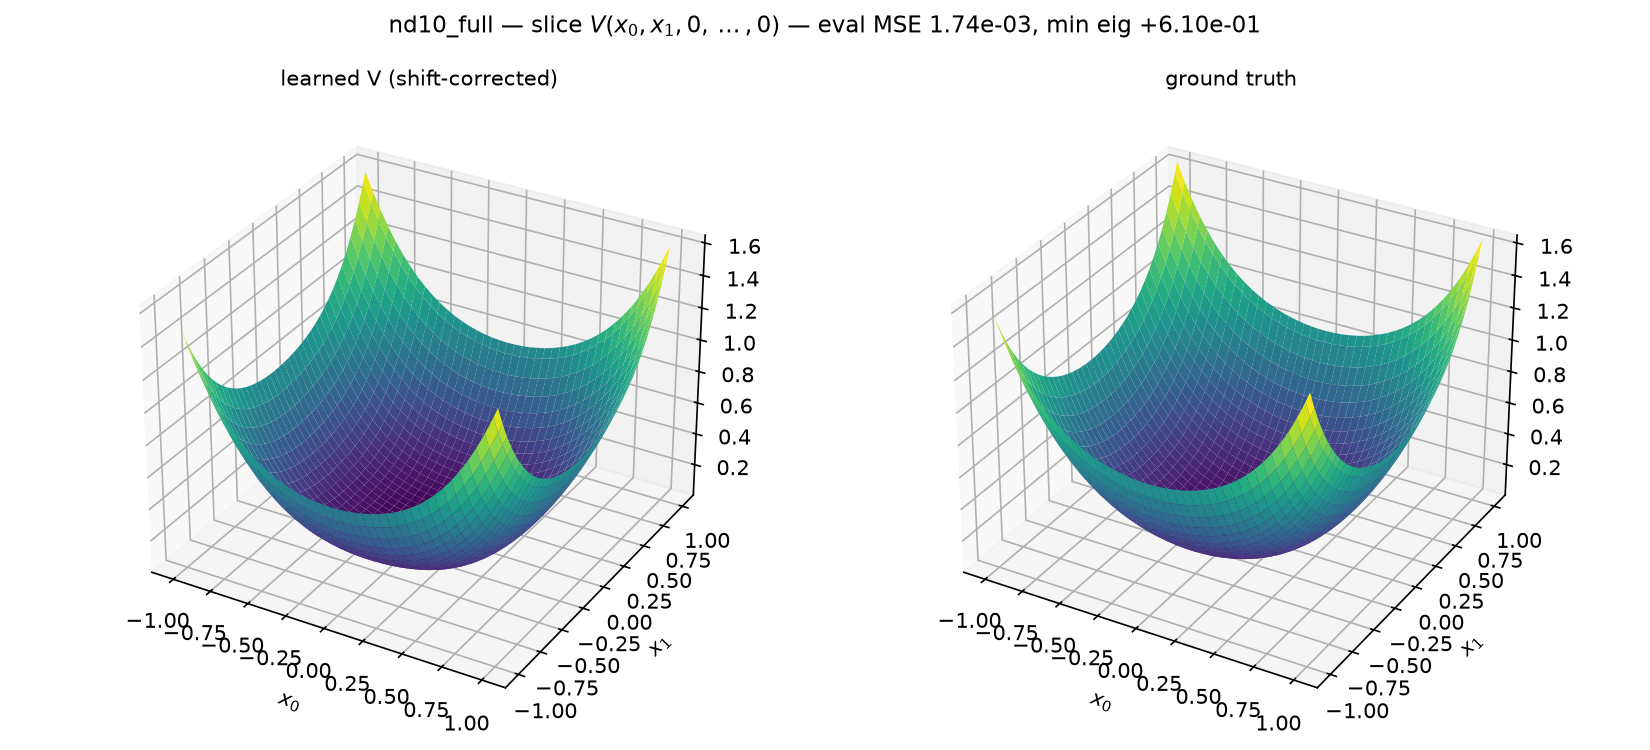
\includegraphics[width=0.95\textwidth]{figures/nd10_slice.png}
  \caption{10D benchmark: the slice $V(x_0, x_1, 0, \dots, 0)$ of the
  learned value function (left) against the ground truth (right).}
  \label{fig:nd10}
\end{figure}

The spurious-solution phenomenon persists in ten dimensions: the
unconstrained control drives the residual to $7\times10^{-6}$ yet lands at
evaluation error $1.53$, non-convex at \emph{every} audited point
(Table~\ref{tab:nd}, first row). The full stack solves the problem
(Table~\ref{tab:nd}, Figure~\ref{fig:nd10}): evaluation MSE
$1.7\times10^{-3}$ ($\approx 1\%$
relative), and the exact-eigenvalue audit finds the learned function
\emph{strictly} convex at every one of the 300 audited points, with minimum
eigenvalue $+0.61$ --- comfortably above the margin and below the true floor
of $1$, consistent with a slightly smoothed approximation of the true
curvature. Accuracy is lower than in 2D ($10^{-3}$ vs $10^{-6}$), as
expected from the fixed network width and the Monte Carlo nature of both the
collocation and the curvature constraint; we did not tune the 10D run.

%=============================================================================
\section{Certified architectures without a penalty}\label{sec:lseq}
%=============================================================================

The soft penalty solves both 2D problems and the 10D problem, but it carries
no hard guarantee: convexity is verified at sampled points after training,
the margin is a tunable loss weight, and the convexity term competes with the
residual during optimization. The ICNN had the opposite profile --- a hard
guarantee, but untrainable through the residual (Section~\ref{sec:icnn}). We
now show these are not the only options: \emph{two} architectures are
\emph{both} convex by construction \emph{and} trainable with no penalty term
at all. The first repairs the ICNN directly; the second changes the function
class.

\paragraph{Diagnosis: why the ICNN constraint, not convexity, was the
problem.} The ICNN failure is often misattributed to convexity being ``only
local'' --- it is not: an ICNN is globally convex on all of $\R^d$, and our
trained ICNNs were strictly convex on the entire test grid. The failure is
the \emph{geometry of the parameterization}. Enforcing $W \ge 0$ by clipping
makes the feasible set a polyhedral cone whose faces trap weights and, under
ReLU, kill units irreversibly (Section~\ref{sec:icnn}); non-negative weights
bias signal propagation toward a single degenerate attractor; and the
skip-free variant is not universal over convex functions. The constraint is a
\emph{sufficient} condition on weights (non-negativity) imposed on a
parameter space hostile to gradient descent, rather than the \emph{actual}
property (a positive semi-definite Hessian) imposed on the output.

\subsection{Fixing the ICNN: skip connections and smooth positivity}
\label{sec:ficnn}

Each item in the diagnosis has an architecture-level remedy, applied without
touching the loss. We take the fully-input-convex network (FICNN) of
\cite{amos2017input} and make three changes:
\begin{enumerate}[itemsep=1pt]
  \item \textbf{Input skip connections} at every layer
        ($z_{l+1} = g(W^z_l z_l + W^x_l x + b_l)$, with $W^z_l \ge 0$ but
        $W^x_l$ \emph{unconstrained}). The passthrough of $x$ is exactly what
        makes ICNNs universal over convex functions; the 2024 variant had
        dropped it.
  \item \textbf{Smooth positivity by reparameterization}: the non-negative
        weight is $\mathrm{softplus}(\rho)$ for an unconstrained $\rho$. There
        is no clipping, hence no trapping faces, and gradients flow through
        every unit at every step.
  \item \textbf{Smooth convex activation} ($g = \mathrm{softplus}$), convex
        and non-decreasing with nowhere-zero derivative, so units cannot die
        as ReLU units do.
\end{enumerate}
An optional $\tfrac{m}{2}\|x\|^2$ term makes the result $m$-strongly convex.
Convexity holds for \emph{any} values of the unconstrained parameters, so the
parameter space is flat and Adam runs unimpeded.

The skip connection is decisive, and a controlled ablation isolates it
(Table~\ref{tab:ficnn}): on LQR2D, with everything else identical (smooth
positivity, softplus activation, anchor), the skip-free FICNN stalls at
evaluation error $1.8\times10^{-2}$ while the skip version reaches
$2.2\times10^{-7}$ --- five orders of magnitude, confirming that the
2024 skip-free failure (Section~\ref{sec:icnn}) was the missing passthrough,
not the convexity constraint. With skips the repaired ICNN solves all three
problems convex-by-construction and penalty-free
(Figure~\ref{fig:ficnn}): NonLinear2D to $4.1\times10^{-3}$ (with
continuation) and the 10D problem to $1.8\times10^{-1}$, both with zero
convexity violations.

A capacity sweep, however, reveals the FICNN's ceiling: on NonLinear2D,
widening the network from 64 to 128 to 256 (depth 3) makes accuracy
\emph{worse}, not better ($4.1\times10^{-3} \to 1.5\times10^{-2} \to
2.3\times10^{-2}$; Figure~\ref{fig:sweeps}, right), and adding a layer does
not help either. The gap to the penalty method is therefore \emph{not} a
capacity limitation but a trainability one: the constrained-weight signal
propagation conditions worse as the network grows --- the well-documented
difficulty of scaling ICNNs that motivated dedicated initialization schemes
\cite{hoedt2023principled}. This contrasts sharply with the next architecture,
whose accuracy improves with size.

\begin{table}[t]
\centering\small
\caption{Repaired ICNN (FICNN), trained on residual + anchor
(+ continuation for the nonlinear cases) with \emph{no} convexity penalty.
The skip ablation (top block) holds everything else fixed.}
\label{tab:ficnn}
\begin{tabular}{llccc}
\toprule
Problem & Variant & Eval.\ MSE & $\min\lammin$ & Viol. \\
\midrule
LQR2D       & FICNN, skip                  & $2.2\times10^{-7}$ & $+0.66$ & 0\% \\
            & FICNN, skip + $m{=}0.05$     & $1.8\times10^{-7}$ & $+0.66$ & 0\% \\
            & FICNN, \emph{no} skip (control) & $1.8\times10^{-2}$ & $0.0$ & stalled \\
\midrule
NonLinear2D & FICNN, skip (+ continuation) & $4.1\times10^{-3}$ & $+0.38$ & 0\% \\
10D cubic   & FICNN, skip (+ continuation) & $1.8\times10^{-1}$ & $+0.10$ & 0\% \\
\bottomrule
\end{tabular}
\end{table}

\begin{figure}[t]
  \centering
  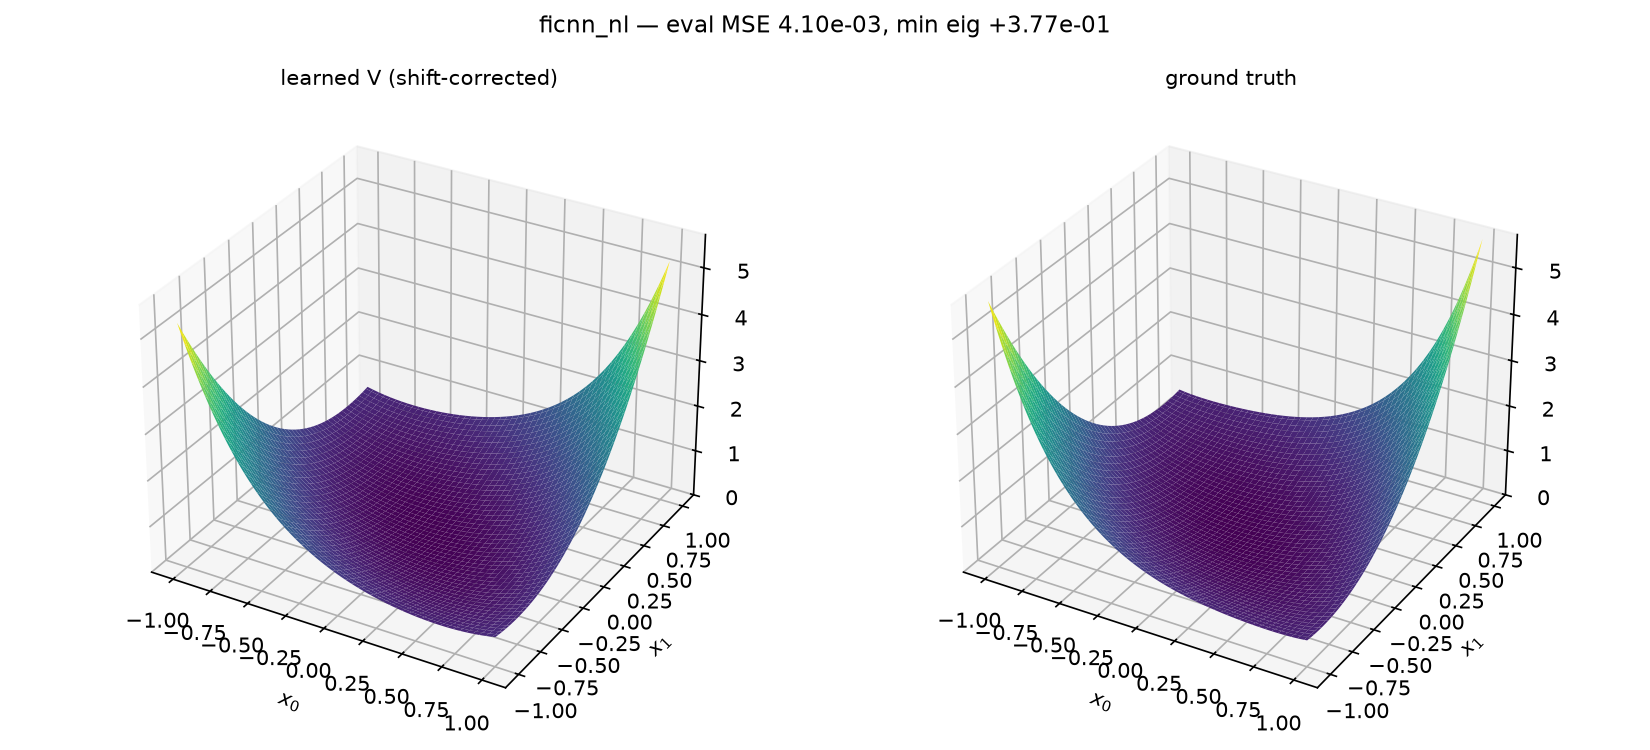
\includegraphics[width=0.95\textwidth]{figures/ficnn_nl.png}
  \caption{Repaired ICNN (FICNN with skip connections, smooth positivity) on
  NonLinear2D, trained with no convexity penalty: learned $V$ (left) vs ground
  truth (right), eval.\ MSE $4.1\times10^{-3}$, convex by construction.}
  \label{fig:ficnn}
\end{figure}

\subsection{Changing the class: log-sum-exp of quadratics}
\label{sec:lseqsub}

A second route abandons weight-sign constraints entirely and builds convexity
into the function form.

\paragraph{Construction.} Place the constraint in the output directly:
\begin{equation}\label{eq:lseq}
  V_\theta(x) \;=\; \frac{m}{2}\|x\|^2
  \;+\; \frac{1}{\tau}\log \sum_{i=1}^{K}
  \exp\!\Big( \tau\,\big( \tfrac12 x^\top L_i L_i^\top x + b_i^\top x + c_i \big) \Big),
\end{equation}
with parameters $\{L_i \in \R^{d\times d}, b_i \in \R^d, c_i \in \R\}$
\emph{unconstrained}. Each component quadratic is convex because
$L_i L_i^\top \succeq 0$ for any $L_i$ (no constraint needed); log-sum-exp is
convex and non-decreasing, so the composition is convex; and the quadratic
prefactor gives, with $p(x) = \mathrm{softmax}(\tau q(x))$,
\begin{equation}
  \nabla^2 V_\theta(x) \;=\; mI + \sum_i p_i(x)\, L_i L_i^\top
  + \tau\,\mathrm{Cov}_{p}\!\big(L_i L_i^\top x + b_i\big)
  \;\succeq\; mI .
\end{equation}
Thus $V_\theta$ is $m$-strongly convex on all of $\R^d$ \emph{by
construction}: the margin is now an architectural constant, not a loss term,
and no convexity penalty is used at all. This is the smooth (log-sum-exp)
form of a max-of-quadratics expansion --- the function class of max-plus
methods for HJB equations \cite{mceneaney2007curse} --- and the induced
feedback law $u^* \propto g^\top \nabla V_\theta = g^\top(mx + \sum_i p_i(x)
(L_i L_i^\top x + b_i))$ is a softmax-gated mixture of linear controllers,
recovering an SDRE-like structure without being told to. At $K=1$ it is
exactly a quadratic, so LQR is representable and $\varepsilon$-continuation
starts inside the class.

\paragraph{Results.} We train \eqref{eq:lseq} with the residual and
equilibrium anchor only --- no convexity penalty --- using the same
continuation schedule as before. Table~\ref{tab:lseq} reports the outcome.
On LQR2D the architecture is \emph{exact}, reaching evaluation MSE
$3.6\times10^{-9}$ --- the best result in this paper, better than the penalty
method --- with the learned Hessian matching the true Riccati value
$P\approx0.69I$. On the nonlinear and 10D problems it solves the problem with
a hard certificate (zero violations by construction, confirmed by exact
eigendecomposition).

\paragraph{Quadratic components, non-quadratic value functions.} A single
quadratic ($K=1$) can only represent an LQR-type value function, so it is
natural to ask whether \eqref{eq:lseq} is limited to quadratic problems. It
is not: the log-sum-exp of $K$ quadratics is a smooth approximation of their
\emph{maximum}, and max-of-quadratics (indeed max-of-affine) is dense in the
convex functions --- the function class of max-plus methods
\cite{mceneaney2007curse}. The $K$-sweep on NonLinear2D, whose true value
function is non-quadratic, makes this concrete (Figure~\ref{fig:sweeps},
left): $K=1$ stalls at evaluation error $3.3\times10^{-2}$ (the pure-quadratic
ansatz, as expected), and accuracy falls by more than two orders of magnitude
as components are added --- $3.0\times10^{-3}$ ($K{=}4$), $1.5\times10^{-4}$
($K{=}16$), saturating near $2\times10^{-4}$ ($K{=}64$). The nonlinear
capability comes precisely from \emph{combining} quadratics; the learned
minimum curvature also descends toward the true floor ($0.52$ at $K{=}1$
toward $0.02$), evidence the larger basis resolves genuine curvature rather
than collapsing onto one piece. Figure~\ref{fig:lseq} shows the surfaces.

\begin{figure}[t]
  \centering
  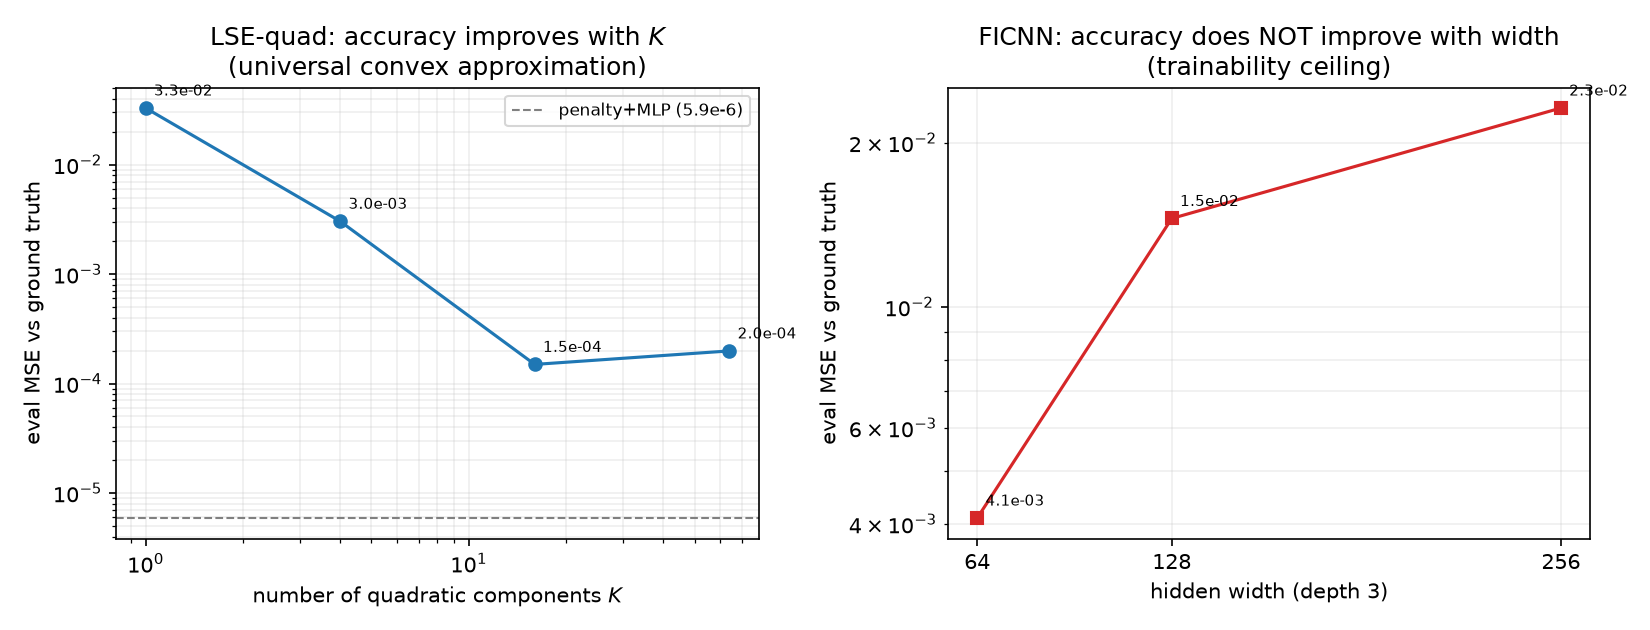
\includegraphics[width=\textwidth]{figures/capacity_sweeps.png}
  \caption{Capacity sweeps on NonLinear2D, both penalty-free and
  convex-by-construction. \textbf{Left:} LSE-quad accuracy improves by orders
  of magnitude as quadratic components $K$ are added ($K{=}1$ is a single
  quadratic and fails), the signature of universal convex approximation.
  \textbf{Right:} the repaired ICNN does \emph{not} improve with width --- a
  trainability ceiling, not a capacity limit. Dashed line: penalty + MLP
  reference.}
  \label{fig:sweeps}
\end{figure}

\begin{table}[t]
\centering\small
\caption{LSE-of-quadratics architecture \eqref{eq:lseq}, trained on residual
+ anchor (+ continuation for the nonlinear cases) with \emph{no} convexity
penalty. Convexity holds by construction; ``Viol.'' is from exact
eigendecomposition and is zero throughout. Penalty-method numbers from
Tables~\ref{tab:lqr}--\ref{tab:nd} shown for comparison.}
\label{tab:lseq}
\begin{tabular}{llccc}
\toprule
Problem & Architecture / method & Eval.\ MSE & $\min\lammin$ & Viol. \\
\midrule
LQR2D       & LSE-quad ($K{=}8$)            & $\mathbf{3.6\times10^{-9}}$ & $+0.69$ & 0\% \\
            & \quad(penalty + MLP, best)   & $2.1\times10^{-8}$ & $+0.62$ & 0\% \\
\midrule
NonLinear2D & LSE-quad ($K{=}1$, quadratic) & $3.3\times10^{-2}$ & $+0.52$ & 0\% \\
            & LSE-quad ($K{=}16$, $\tau{=}2$) & $1.5\times10^{-4}$ & $+0.28$ & 0\% \\
            & \quad(penalty + MLP, best)   & $5.9\times10^{-6}$ & $+0.02$ & 0\% \\
\midrule
10D cubic   & LSE-quad ($K{=}8$)           & $5.6\times10^{-2}$ & $+0.57$ & 0\% \\
            & LSE-quad ($K{=}32$, $\tau{=}4$) & $2.9\times10^{-2}$ & $+0.98$ & 0\% \\
            & \quad(penalty + MLP)         & $1.7\times10^{-3}$ & $+0.61$ & 0\% \\
\bottomrule
\end{tabular}
\end{table}

\begin{figure}[t]
  \centering
  \begin{subfigure}[b]{0.95\textwidth}
    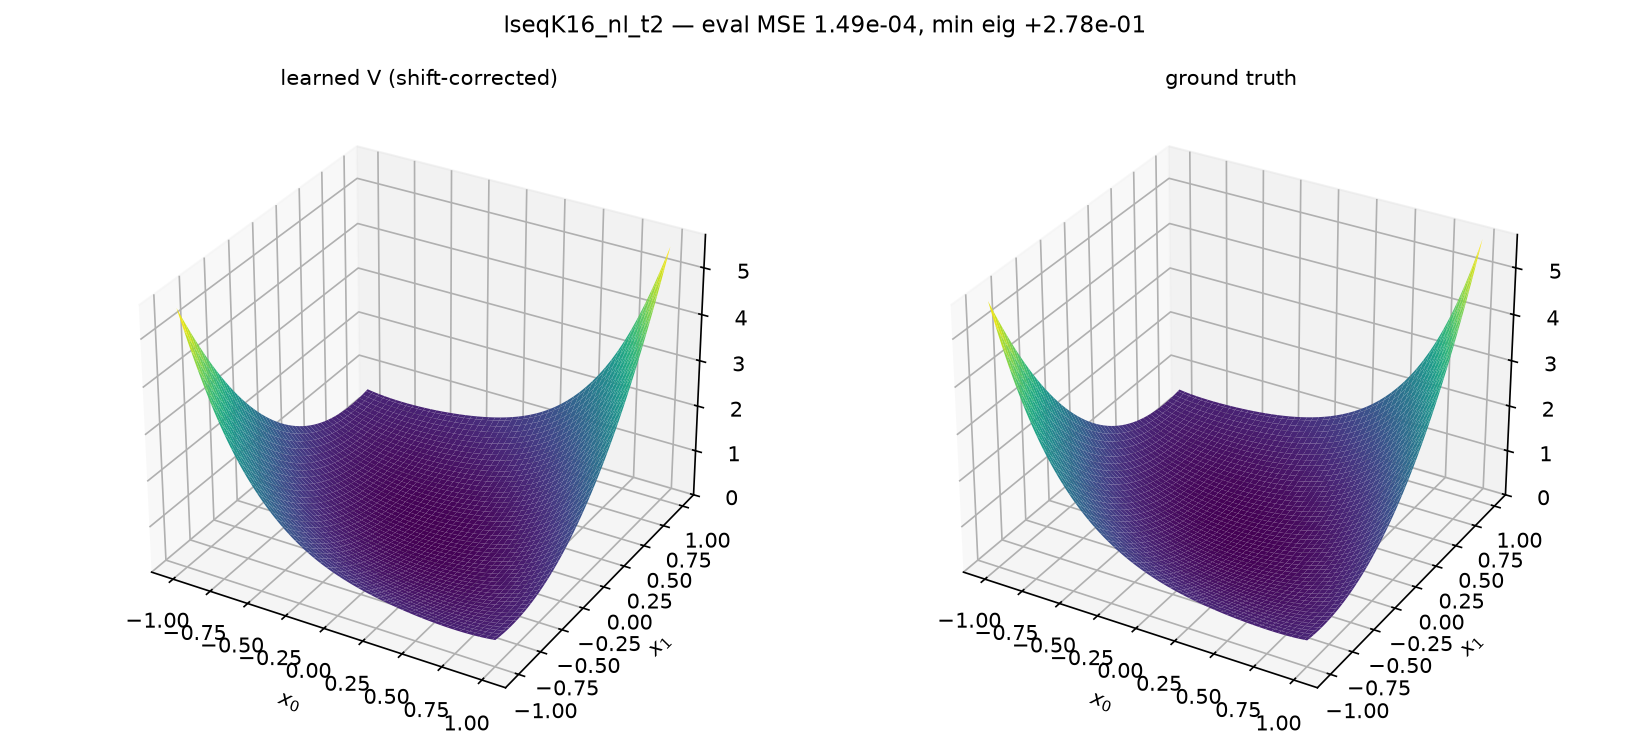
\includegraphics[width=\textwidth]{figures/lseq_nl.png}
    \caption{NonLinear2D, $K=16$: eval.\ MSE $1.5\times10^{-4}$.}
  \end{subfigure}\\[1ex]
  \begin{subfigure}[b]{0.95\textwidth}
    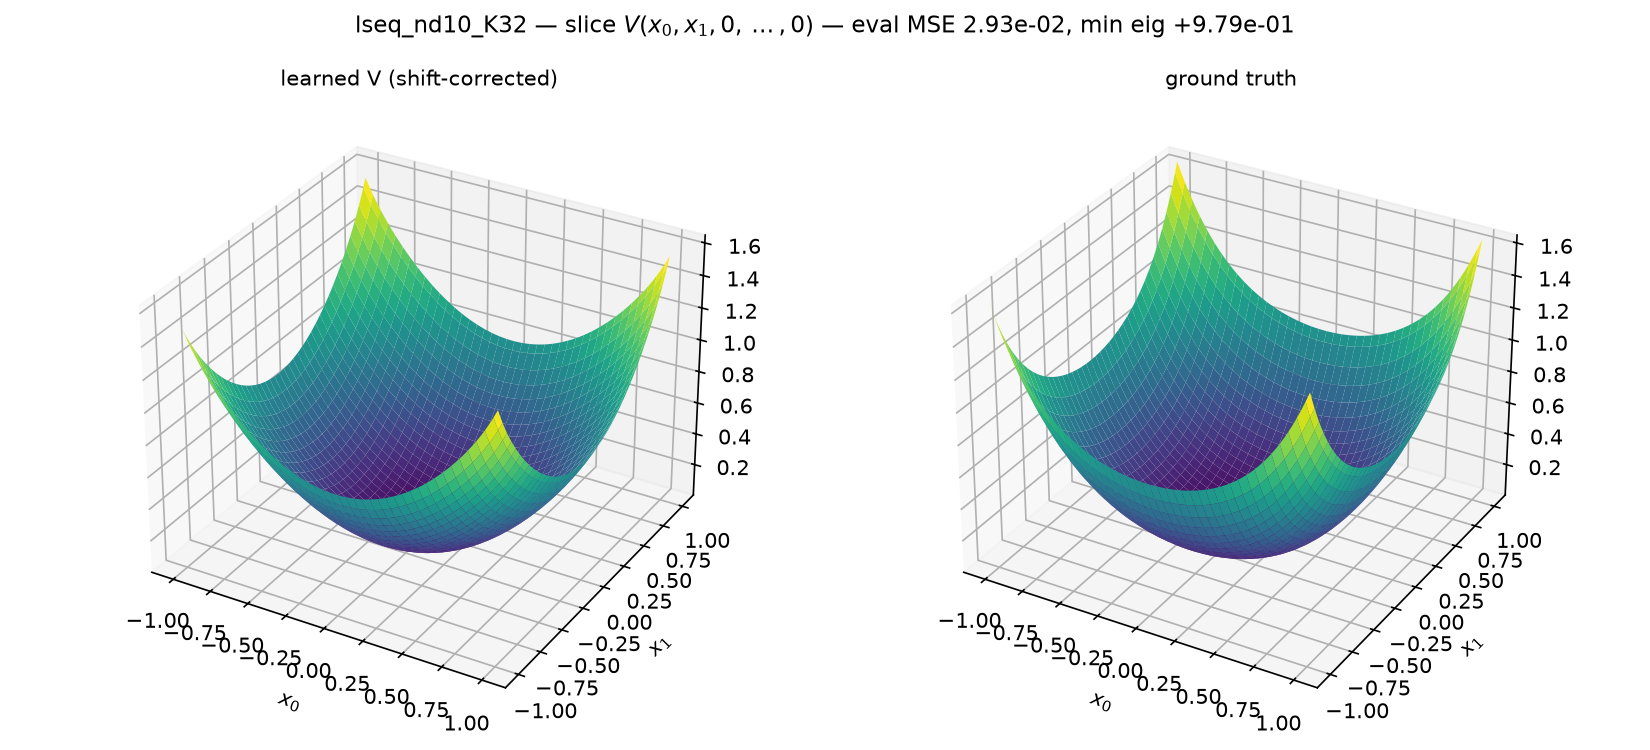
\includegraphics[width=\textwidth]{figures/lseq_nd10_slice.png}
    \caption{10D, $K=32$: slice $V(x_0, x_1, 0, \dots, 0)$, eval.\ MSE
    $2.9\times10^{-2}$.}
  \end{subfigure}
  \caption{LSE-of-quadratics architecture (left panels) vs ground truth
  (right panels), trained with no convexity penalty.}
  \label{fig:lseq}
\end{figure}

Residual risks specific to \eqref{eq:lseq}: a softmax temperature $\tau$ that
may need annealing to avoid gating collapse (another homotopy), and an
$O(Kd^2)$ parameter count that motivates low-rank $L_i$ in high dimension.

\subsection{Which route?}\label{sec:which}

Table~\ref{tab:archcompare} places the three convexity mechanisms side by
side. All three give a convex value function; they trade accuracy against the
strength of the guarantee. The soft penalty is the most accurate everywhere
(it constrains an otherwise-unconstrained MLP, the most expressive model), but
certifies convexity only at sampled points. The two architectures certify by
construction --- zero violations provable, no margin to tune --- and the
LSE-of-quadratics is the most accurate of them (exact on LQR), while the
repaired ICNN is the most faithful to the standard convex-network literature.
The architectures cost one to three orders of accuracy on value functions far
from piecewise-quadratic, at the $K$ and widths tested. The practical reading:
use the penalty when raw accuracy dominates, an architecture when a hard
certificate or interpretability does, or distil a penalty-trained solution
into an architecture to obtain both.

\begin{table}[t]
\centering\small
\caption{The three convexity mechanisms, eval.\ MSE against ground truth.
Penalty: soft Hessian-eigenvalue hinge on an unconstrained MLP, convexity
verified at samples. FICNN / LSE-quad: convex by construction (zero violations
provable), trained with no penalty. All use the equilibrium anchor and, for
the nonlinear cases, $\varepsilon$-continuation.}
\label{tab:archcompare}
\begin{tabular}{lccc}
\toprule
 & Penalty + MLP & FICNN (repaired ICNN) & LSE-quad \\
 & (verified at samples) & (certified) & (certified) \\
\midrule
LQR2D       & $2.1\times10^{-8}$ & $2.2\times10^{-7}$ & $\mathbf{3.6\times10^{-9}}$ \\
NonLinear2D & $\mathbf{5.9\times10^{-6}}$ & $4.1\times10^{-3}$ & $1.5\times10^{-4}$ \\
10D cubic   & $\mathbf{1.7\times10^{-3}}$ & $1.8\times10^{-1}$ & $2.9\times10^{-2}$ \\
\bottomrule
\end{tabular}
\end{table}

%=============================================================================
\section{Discussion: pros and cons of each route}\label{sec:discussion}
%=============================================================================

\subsection{Summary of approaches}

Table~\ref{tab:proscons} collects the trade-offs of every approach tried,
from the published two-pass baseline through each ingredient of the one-pass
recipe.

\begin{table}[h]
\centering\small
\caption{Qualitative comparison of all approaches tried.}
\label{tab:proscons}
\begin{tabularx}{\textwidth}{lXX}
\toprule
Approach & Pros & Cons \\
\midrule
Two-pass (SDRE data $\to$ residual) \cite{borovykh2022data} &
Robust; data places the network in the right basin; published baseline. &
Requires problem-specific data generation; SDRE itself is $7.6\times10^{-3}$
from the truth here; two training stages. \\
\addlinespace
Hard ICNN (skip-free) &
Provable convexity certificate; zero violations by construction. &
Not trainable through the residual on our benchmarks: dying units (ReLU),
degenerate attractor, or a $6\times10^{-3}$ residual plateau; ReLU variant
passes the convexity check vacuously. \\
\addlinespace
Repaired ICNN (FICNN: skip + smooth positivity) &
Hard certificate; trainable (skip ablation: $1.8\times10^{-2}\to
2.2\times10^{-7}$ on LQR); stays within the standard convex-network family;
unconstrained parameters. &
Least accurate of the three convex methods on far-from-quadratic value
functions ($4\times10^{-3}$ / $1.8\times10^{-1}$ on NL2D / 10D). \\
\addlinespace
LSE-of-quadratics architecture &
Hard certificate \emph{and} trainable (unconstrained parameters); exact on
LQR ($3.6\times10^{-9}$); margin is an architectural constant; interpretable
mixture-of-feedbacks controller. &
1--3 orders less accurate than penalty+MLP on far-from-quadratic value
functions at the $K$ tested; $O(Kd^2)$ parameters; $\tau$ may need annealing
to avoid gating collapse. \\
\addlinespace
Output hinge penalty + margin &
Full expressivity of unconstrained nets; margin acts as solution selection;
exact on LQR; simple (one weight, one margin). &
No hard certificate (grid verification only); margin must lie below the true
curvature floor, which may be unknown; $O(d^3)$ eigenvalue cost beyond
closed-form 2D. \\
\addlinespace
Augmented Lagrangian variant &
Principled constraint handling; works comparably ($8.9\times10^{-6}$). &
More machinery (multiplier state, update schedule) with no measured gain
over the fixed hinge. \\
\addlinespace
Equilibrium anchor &
Free (problem knowledge, not data); removes shift indeterminacy; improved
LQR by an order of magnitude. &
Insufficient alone --- anchored unconstrained runs still pick spurious
branches. \\
\addlinespace
Warm shaping ($\tfrac12\|x\|^2$ pre-fit) &
Data-free; cheap. &
No measurable effect on the plateau. \\
\addlinespace
Collocation resampling &
Removes a genuine $100\times$ off-sample residual gap; standard practice. &
Does not by itself remove spurious branches. \\
\addlinespace
$\varepsilon$-homotopy continuation &
Breaks the optimization plateau ($1.2 \to 6\times10^{-6}$); data-free;
conceptually principled (tracks a continuous solution path from a solvable
base problem). &
Requires a natural homotopy parameter; anneal schedule is a hyperparameter;
path-following has no formal guarantee here. \\
\bottomrule
\end{tabularx}
\end{table}

\subsection{Why the pieces compose}
The ablation trail supports a clean division of labor:
\emph{the convexity margin decides which solution; continuation provides the
path to it; the anchor fixes the gauge; resampling makes the residual mean
what it claims}. Removing any one ingredient reproduces a specific failure:
no penalty $\to$ spurious branch at near-zero residual; no margin $\to$
partial convexity violations and a $4.9\times10^{-3}$ floor; no continuation
$\to$ the $3\times10^{-2}$ plateau; no resampling $\to$ collocation
overfitting.

\subsection{Limitations}
\begin{enumerate}[itemsep=1pt]
  \item \textbf{Dimensionality.} The directional-curvature penalty scales
        the method to 10D (Section~\ref{sec:nd}), but enforces the spectral
        constraint only in expectation; its sample complexity in still
        higher dimension, and the accuracy gap vs 2D ($10^{-3}$ vs
        $10^{-6}$), are unquantified.
  \item \textbf{Margin selection.} The margin must lie below the true
        curvature floor. We used known floors ($0.02$ in 2D, $1$ in 10D);
        without them one would anneal the margin or estimate the floor on
        the fly. A principled rule is open.
  \item \textbf{Certificate vs accuracy.} The penalty method verifies
        convexity only at sampled points; the LSE-of-quadratics architecture
        (Section~\ref{sec:lseq}) gives a hard certificate but is less
        accurate on far-from-quadratic value functions at the $K$ tested.
        Closing this gap --- larger or low-rank $K$, $\tau$ annealing, or
        distilling a penalty-trained solution into the architecture for both
        accuracy and a certificate --- remains open.
  \item \textbf{Statistical strength.} Key comparisons rest on 1--3 seeds.
        The LQR result is confirmed on three seeds; the continuation and
        10D results on one seed each (the former on two constraint
        mechanisms).
  \item \textbf{Scope of the convexity prior.} The method targets problems
        whose value function is convex on the domain of interest --- a
        property that can and should be checked in advance, as done for
        Cucker--Smale in Section~\ref{sec:cs}, where it fails. For such
        problems a convexity-region restriction or a convex-plus-correction
        decomposition is needed; both are open.
\end{enumerate}

%=============================================================================
\section{Conclusion}
%=============================================================================

The data pass of \cite{borovykh2022data} can be removed. Its role ---
selecting the physically correct solution among the many functions that
satisfy the stationary HJB residual --- is taken over by structural priors
that cost nothing to state: convexity with a strong-convexity margin,
equilibrium anchoring, and homotopy from a solvable base problem. On both
benchmarks the resulting one-pass solver is not merely competitive with the
two-pass baseline; it is more accurate than the SDRE data that the two-pass
scheme trains on, by three orders of magnitude on the nonlinear problem.

The recipe scales: with the directional-curvature penalty in place of the
closed-form eigenvalue, a ten-dimensional nonlinear problem with provably
convex value function is solved to $\approx 1\%$ relative error, strictly
convex at every audited point. The scope is also now delimited: the
Cucker--Smale value function is demonstrably non-convex in the domain
interior, so flocking problems require an extension --- a convexity-region
restriction or a convex-plus-correction decomposition --- rather than the
method as-is.

Two routes deliver the convexity prior: a soft Hessian-eigenvalue penalty,
most accurate but verified only at samples; and a log-sum-exp-of-quadratics
architecture that is strongly convex by construction over unconstrained
parameters, exact on LQR and certified everywhere, at some cost in accuracy.
The architecture also clarifies the ICNN's failure: convexity was never the
obstacle (an ICNN is globally convex), the weight-space constraint geometry
was.

The immediate next steps are: a margin-selection rule; closing the
architecture's accuracy gap (low-rank or larger $K$, $\tau$ annealing, or
distilling a penalty-trained solution into the architecture for accuracy and
a certificate at once); the skip-connected ICNN control experiment; tuning
and seed replication of the 10D result; and the convex-plus-correction
extension toward Cucker--Smale. On the theory side, the empirical division of
labor
--- convexity as solution selection, continuation as path-finding ---
invites a uniqueness result for strongly convex, anchored solutions of
\eqref{eq:hjb}, and connects to continuation theorems studied in the
companion work on Riemannian gradient smoothing (in preparation).

%=============================================================================
\begin{thebibliography}{9}

\bibitem{raissi2019physics}
M.~Raissi, P.~Perdikaris, G.E.~Karniadakis.
\newblock Physics-informed neural networks: A deep learning framework for
solving forward and inverse problems involving nonlinear partial
differential equations.
\newblock \emph{Journal of Computational Physics}, 378:686--707, 2019.

\bibitem{borovykh2022data}
A.~Borovykh, D.~Kalise, A.~Laignelet, P.~Parpas.
\newblock Data-driven initialization of deep learning solvers for
Hamilton--Jacobi--Bellman PDEs.
\newblock \emph{IFAC-PapersOnLine}, 55(30):168--173, 2022.

\bibitem{amos2017input}
B.~Amos, L.~Xu, J.Z.~Kolter.
\newblock Input convex neural networks.
\newblock \emph{Proceedings of the 34th International Conference on Machine
Learning (ICML)}, PMLR 70:146--155, 2017.

\bibitem{hoedt2023principled}
P.-J.~Hoedt, G.~Klambauer.
\newblock Principled weight initialisation for input-convex neural networks.
\newblock \emph{Advances in Neural Information Processing Systems
(NeurIPS)}, 2023.

\bibitem{banks2007nonlinear}
H.T.~Banks, B.M.~Lewis, H.T.~Tran.
\newblock Nonlinear feedback controllers and compensators: a
state-dependent Riccati equation approach.
\newblock \emph{Computational Optimization and Applications},
37(2):177--218, 2007.

\bibitem{mceneaney2007curse}
W.M.~McEneaney.
\newblock A curse-of-dimensionality-free numerical method for solution of
certain HJB PDEs.
\newblock \emph{SIAM Journal on Control and Optimization},
46(4):1239--1276, 2007.

\bibitem{allgower1990numerical}
E.L.~Allgower, K.~Georg.
\newblock \emph{Numerical Continuation Methods: An Introduction}.
\newblock Springer, 1990.

\bibitem{bardi1997optimal}
M.~Bardi, I.~Capuzzo-Dolcetta.
\newblock \emph{Optimal Control and Viscosity Solutions of
Hamilton--Jacobi--Bellman Equations}.
\newblock Birkh\"auser, 1997.

\end{thebibliography}

\end{document}
